\beginsong{And're, die das Land so sehr nicht liebten}[
    txt={Theodor Kramer}, 
    txtjahr={1938}
    mel={Erich Schmeckenbecher},
    meljahr={1979}, 
    bo={30}, 
    pfii={84}, 
    gruen={191}, 
    siru={20},
]

\beginverse
\endverse
\centering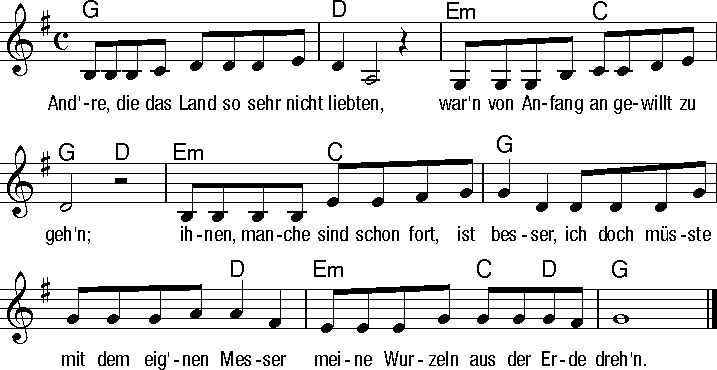
\includegraphics[width=1\textwidth]{Noten/Lied005.pdf}	

\beginverse
\[G]Keine Nacht hab' ich seither ge\[D]schlafen, 
\[Em]und es ist mir \[C]mehr als weh zu\[G]mut.\[D]
\[Em]Viele Wochen \[C]sind seither ver\[G]strichen, 
alle Kraft ist längst aus mir ge\[D]wichen,
\[Em]und ich fühl', dass \[C]ich dar\[D]an ver\[G]blut'.
\endverse

\beginverse
^Und doch müsst' ich mich von hinnen ^heben, 
^sei's auch nur zu ^bleiben, was ich ^war.^
^Nimmer kann ich, ^wo ich bin, ge^deihen, 
draußen braucht ich wahrlich nicht zu ^schreien,
^denn mein leises ^Wort war ^immer ^wahr.
\endverse

\beginverse
^Seiner wär' ich wie in alten ^Tagen 
^sicher, schluchzend ^wider mich ge^wandt. ^
^Hätt' ich Tag und ^Nacht mich nur zu ^heißen, 
mich samt meinen Wurzeln auszu^reißen
^und zu setzen ^in ein ^and'res ^Land. 
\endverse

\endsong

\beginscripture{}
Kramer beschäftigte sich hauptsächlich mit gesellschaftlichen Außenseitern und verfasste so über 10.000 Werke, von denen viele unveröffentlicht sind. Dieses Lied fand jedoch Einzug in das Fahrtenbuch der Wandervögel ''Der Zupfgeigenhansel''.
\endscripture
